%%%%%%%%%%%%%%%%%%%%%%%%%%%%%%%%%%%%%%%%%
% Beamer Presentation
% LaTeX Template
% Version 1.0 (10/11/12)
%
% This template has been downloaded from:
% http://www.LaTeXTemplates.com
%
% License:
% CC BY-NC-SA 3.0 (http://creativecommons.org/licenses/by-nc-sa/3.0/)
%
%%%%%%%%%%%%%%%%%%%%%%%%%%%%%%%%%%%%%%%%%

%----------------------------------------------------------------------------------------
%	PACKAGES AND THEMES
%----------------------------------------------------------------------------------------

\documentclass{beamer}

\mode<presentation> {

% The Beamer class comes with a number of default slide themes
% which change the colors and layouts of slides. Below this is a list
% of all the themes, uncomment each in turn to see what they look like.

% \usetheme{default}
% \usetheme{AnnArbor}
% \usetheme{Antibes}
% \usetheme{Bergen}
% \usetheme{Berkeley}
% \usetheme{Berlin}
\usetheme{Boadilla}
% \usetheme{CambridgeUS}
% \usetheme{Copenhagen}
% \usetheme{Darmstadt}
% \usetheme{Dresden}
% \usetheme{Frankfurt}
% \usetheme{Goettingen}
% \usetheme{Hannover}
% \usetheme{Ilmenau}
% \usetheme{JuanLesPins}
% \usetheme{Luebeck}
% \usetheme{Madrid}
% \usetheme{Malmoe}
% \usetheme{Marburg}
% \usetheme{Montpellier}
% \usetheme{PaloAlto}
% \usetheme{Pittsburgh}
% \usetheme{Rochester}
% \usetheme{Singapore}
% \usetheme{Szeged}
% \usetheme{Warsaw}

% As well as themes, the Beamer class has a number of color themes
% for any slide theme. Uncomment each of these in turn to see how it
% changes the colors of your current slide theme.

% \usecolortheme{albatross}
% \usecolortheme{beaver}
% \usecolortheme{beetle}
% \usecolortheme{crane}
\usecolortheme{dolphin}
% \usecolortheme{dove}
% \usecolortheme{fly}
% \usecolortheme{lily}
% \usecolortheme{orchid}
% \usecolortheme{rose}
% \usecolortheme{seagull}
% \usecolortheme{seahorse}
% \usecolortheme{whale}
% \usecolortheme{wolverine}
% \usecolortheme{owl}
%\setbeamertemplate{footline} % To remove the footer line in all slides uncomment this line
%\setbeamertemplate{footline}[page number] % To replace the footer line in all slides with a simple slide count uncomment this line

%\setbeamertemplate{navigation symbols}{} % To remove the navigation symbols from the bottom of all slides uncomment this line

\setbeamertemplate{caption}[numbered]
}

\usepackage{graphicx} % Allows including images
\usepackage{booktabs} % Allows the use of \toprule, \midrule and \bottomrule in tables
\usepackage{caption}
\usepackage{subcaption}
\usepackage{adjustbox}
\usepackage{listings}
\usepackage{color}
\usepackage{cleveref}

\definecolor{mygreen}{rgb}{0,0.6,0}
\definecolor{mygray}{rgb}{0.5,0.5,0.5}
\definecolor{mymauve}{rgb}{0.58,0,0.82}

\lstset{
  basicstyle=\footnotesize\ttfamily,
  breakatwhitespace=false,         % sets if automatic breaks should only happen at whitespace
  breaklines=false,                 % sets automatic line breaking
  captionpos=b,                    % sets the caption-position to bottom
  commentstyle=\color{mygreen},    % comment style
  deletekeywords={...},            % if you want to delete keywords from the given language
  escapeinside={\%*}{*)},          % if you want to add LaTeX within your code
  extendedchars=true,              % lets you use non-ASCII characters; for 8-bits encodings only, does not work with UTF-8
  firstnumber=1,                   % start line enumeration with line 1000
  % frame=single,	                   % adds a frame around the code
  keepspaces=true,                 % keeps spaces in text, useful for keeping indentation of code (possibly needs columns=flexible)
  keywordstyle=\color{blue},       % keyword style
  language=C++,                    % the language of the code
  morekeywords={__global__, __shared__, __device__, __host__, __syncthreads},  % if you want to add more keywords to the set
  numbers=left,                    % where to put the line-numbers; possible values are (none, left, right)
  numbersep=5pt,                   % how far the line-numbers are from the code
  numberstyle=\tiny\color{mygray}, % the style that is used for the line-numbers
  % rulecolor=\color{black},         % if not set, the frame-color may be changed on line-breaks within not-black text (e.g. comments (green here))
  showspaces=false,                % show spaces everywhere adding particular underscores; it overrides 'showstringspaces'
  showstringspaces=false,          % underline spaces within strings only
  showtabs=false,                  % show tabs within strings adding particular underscores
  stepnumber=1,                    % the step between two line-numbers. If it's 1, each line will be numbered
  stringstyle=\color{mymauve},     % string literal style
  tabsize=2,	                   % sets default tabsize to 2 spaces
  title=\lstname                   % show the filename of files included with \lstinputlisting; also try caption instead of title
}

%----------------------------------------------------------------------------------------
%	TITLE PAGE
%----------------------------------------------------------------------------------------

\title[GP on GPUs]{Fast Symbolic Regression on GPUs} % The short title appears at the bottom of every slide, the full title is only on the title page

\author[shortname]{Vimarsh Sathia \inst{1} \and G. Venkatramana \inst{2} \and Thejaswi. N. S \inst{2} } % Your name
\institute[shortinst] % Your institution as it will appear on the bottom of every slide, may be shorthand to save space
{
\inst{1} Indian Institute of Technology Madras \and
\inst{2} Nvidia Corporation % Your institution for the title page
% \medskip
% \textit{cs17b046@cse.iitm.ac.in} % Your email address
}
\date[\today]{Team Presentation \\ \today} % Date, can be changed to a custom date
\logo{
  
\includegraphics[height=1cm]{images/IIT_Madras_Logo.png}~
  
\includegraphics[height=1cm]{images/nvidia.jpg}
}

% clear problem statement, related work and how the work differs from it, main contributions, proofs / results / experimental evaluation, analysis of results / implications of results.

% \AtBeginSection[]
% {
%   \begin{frame}
%       \frametitle{Table of Contents}
%       \tableofcontents[currentsection]
%   \end{frame}
% }
\begin{document}

\begin{frame}
\titlepage % Print the title page as the first slide
\end{frame}

\begin{frame}
\frametitle{Table of Contents} % Table of contents slide, comment this block out to remove it
\tableofcontents
\end{frame}

%----------------------------------------------------------------------------------------
%	PRESENTATION SLIDES
%----------------------------------------------------------------------------------------

\begin{frame}
  \frametitle{NVAITC India Pillars}
  \begin{columns}[t,onlytextwidth]
    \begin{column}{0.3\textwidth}
      \textbf{Establish AI for Science}

      { \footnotesize
        \begin{itemize}
            \item Why? HPC is still key workload in India Supercomputing. India is at stage of redefinition of HPC to AI. 
            \item How? AI for Science Curriculum and Teaching Kit, AI for Science Ambassadors
            \item Where? Tier 1 IIT
        \end{itemize}
      }
    \end{column}
    
    \begin{column}{0.3\textwidth}
      \textbf{Nvidia Products Enhancements}
      { \footnotesize
      \begin{itemize}
        \item Why? Make Researchers part of the Nvidia product 
        \item How? NVAITC Research project to extend Nvidia frameworks
        \item Where? Tier 1 IIT
      \end{itemize}
      }
    \end{column}

    \begin{column}{0.3\textwidth}
      \textbf{Map to AI Nation, Exascale strategy}
      { \footnotesize
        \begin{itemize}
            \item Why? Nvidia pursued as technical research partner and not a vendor. 
            \item How? Establish NVAITC Tech Center at key execution agency
            \item Where? CDAC, IIT
        \end{itemize}
      }
    \end{column}
\end{columns}
\end{frame}
%------------------------------------------------
\section{Introduction}
%------------------------------------------------

\begin{frame}
  \frametitle{A General Outlook}
  Genetic Programming(GP) is a technique which involves the \textit{evolution} of \textit{computer programs}. It is based on the principle of natural selection.\\~\\

  A given \textit{program} population usually is evolved into a new(hopefully better) population using the following $3$ steps:
  \begin{enumerate}
    \item Selection
    \item Mutation
    \item Evaluation --- Usually the bottleneck
  \end{enumerate}
  ~\\
  When using GP to perform Symbolic Regression, the underlying \textit{program} is usually a mathematical equation.
\end{frame}
    
\begin{frame}
  \frametitle{Programs: A Symbolic Regression view}
  \begin{columns}[c]
    \column{0.45\textwidth}
    \begin{itemize}
      \item Denotes a structured mathematical equation. 
      \item GP mostly uses syntax trees to represent solutions. 
      % \begin{align*}
      %   a*a + b \equiv (+ * a a b)
      % \end{align*}
      \item In our implementation, programs are represented using prefix-expression lists
    \end{itemize}

    \column{0.5\textwidth}
    \begin{figure}[h]
      \centering
      \includegraphics[scale=0.5]{images/graphviz/simp_ast.dot.pdf}
      \caption{GP syntax tree representing $a*a+b$. It's prefix form is $(+ * a a b)$.}
      \label{fig:simpast}
    \end{figure}
  \end{columns}
\end{frame}

%------------------------------------------------

\subsection{Problem Statement}

\begin{frame}
  \frametitle{What is the problem?}
  For large input datasets, the evaluation step of the GP algorithm is a well-known bottleneck, and can result in a significant increase in training time. \\~\\
  Our goal is to reduce the training time of GP programs (for symbolic regression) by parallelizing the whole evolution process using GPUs. \\~\\
  
  In order to achieve the above goal, we parallelize the selection and evaluation steps of the GP algorithm using CUDA. \\~\\
  
  Our work has been added as a new algorithm in the \texttt{cuML} library, a GPU accelerated subset of the \texttt{scikit-learn} machine learning library.
\end{frame}

%------------------------------------------------

\subsection{Generational GP Algorithm}

\begin{frame}
  \frametitle{The GP Algorithm}
  Programs are evolved for multiple generations, using the following steps in every generation. 
  \begin{enumerate}
    \item Selection --- Programs to be evolved are chosen based on fitness values. Popular selection methods include tournament, ranking, proportionate and genitor selections.
    \item Mutation --- Denotes the genetic operations on the selected programs. Some common mutation operations are crossover, subtree, hoist and point mutations.
    \item Evaluation --- Denotes the fitness value computation step (on the input dataset) for the new programs. Metrics like Mean Square Error(MSE) are usually used as fitness(loss) functions for a given population in symbolic regression.
  \end{enumerate}
\end{frame}

\begin{frame}
  \frametitle{Initial Population}
  There are $3$ popular initialization methods for program trees in GP
  \begin{itemize}
    \item \textbf{Full} --- All trees are of maximum depth, with only leaves as terminals.
    \item \textbf{Grow} --- Terminals are present at smaller depths, resulting in trees of various sizes.
    \item \textbf{Ramped half-and-half} --- One half of the population is initialized using the Full method, and the other half is initialized using Grow.
  \end{itemize}
  ~\\
  We now explore some common mutations.
\end{frame}
\begin{frame}
  \frametitle{Crossover}
  \begin{columns}
    \begin{column}{0.3\textwidth}
      Crossover mutations are characterized as follows:
      \begin{itemize}
        \item Randomly choose a subtree from both parent and donor. 
        \item Replace parent subtree with donor subtree.
      \end{itemize}
    \end{column}

    \begin{column}{0.6\textwidth}
      \begin{figure}
        \centering
        \begin{subfigure}{0.6\textwidth}
          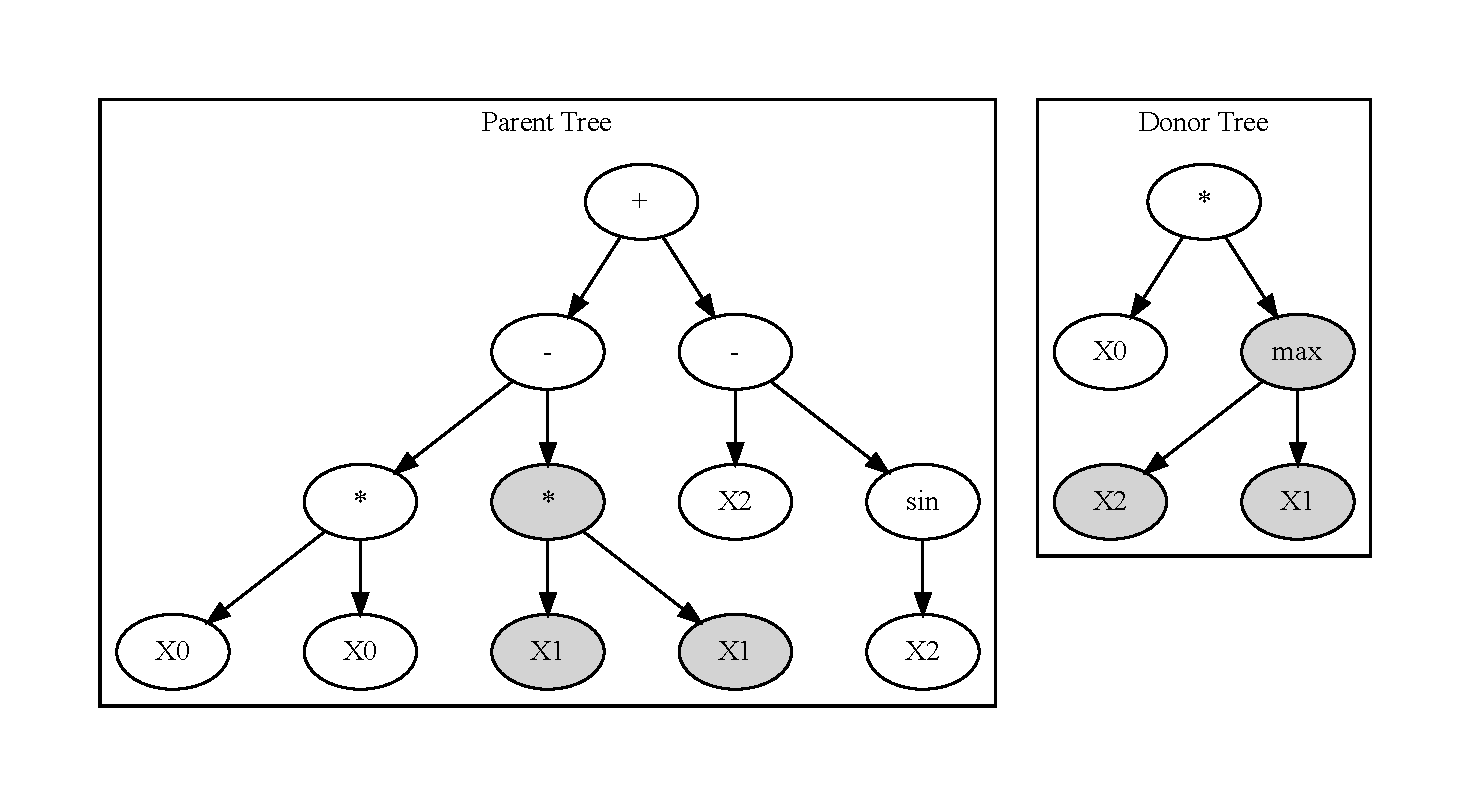
\includegraphics[scale=0.21]{images/graphviz/crossover_before.dot.pdf}
          \caption{Parent and donor tree}
          \label{fig:crossover_muta}
        \end{subfigure}%
        \\
        \begin{subfigure}{0.6\textwidth}
          \centering
          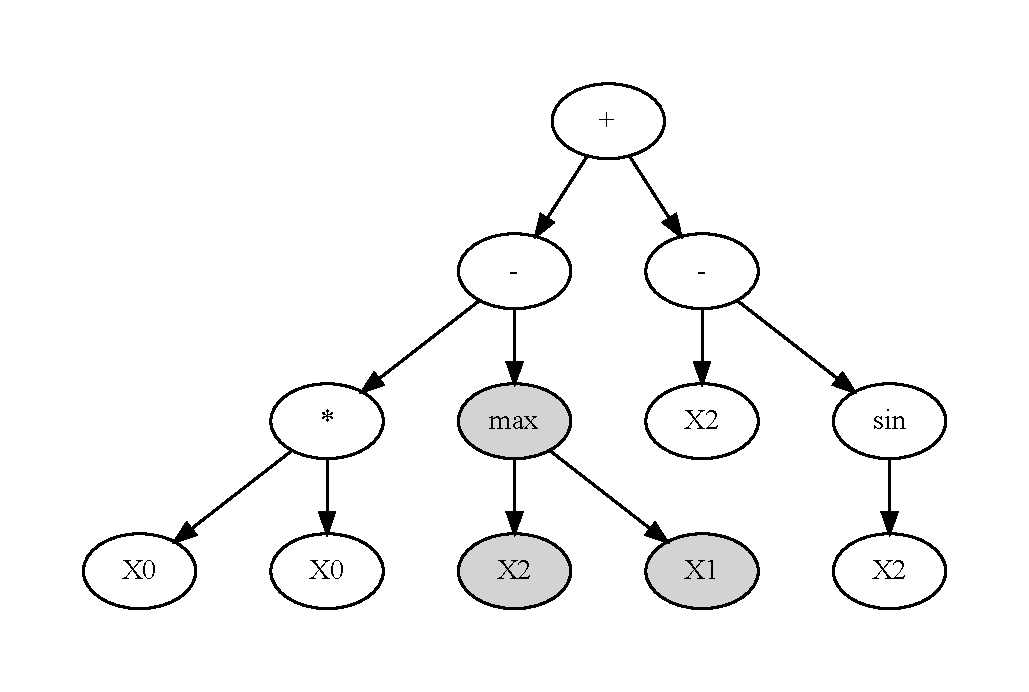
\includegraphics[scale=0.21]{images/graphviz/crossover_after.dot.pdf}
          \caption{Final child tree.}
          \label{fig:crossover_mutb}
        \end{subfigure}
        \caption{Visualizing crossover mutations.}
        \label{fig:crossover}
      \end{figure}
    \end{column}
  \end{columns}
\end{frame}

\begin{frame}
  \frametitle{Subtree Mutations}
  Subtree mutations (a.k.a. headless chicken mutations) are characterized as follows:
  \begin{itemize}
    \item Choose a parent subtree.
    \item Replace it with randomly generated subtree.
  \end{itemize}
  ~\\
  This is the same as a crossover with a random program as donor.\\~\\
  This mutation reintroduces new terminals and extinct functions into the population.
\end{frame}

\begin{frame}
  \frametitle{Hoist Mutations}
  \begin{columns}
    \begin{column}{0.33\textwidth}
      Hoist Mutations can be characterized as follows:
      \begin{itemize}
        \item Choose a subtree of the parent. 
        \item Replace it with a subtree of the chosen subtree.
      \end{itemize}
      This helps reduce bloat in programs.
    \end{column}
    \begin{column}{0.6\textwidth}
      \begin{figure}
        \centering
        \begin{subfigure}{0.6\textwidth}
          \centering
          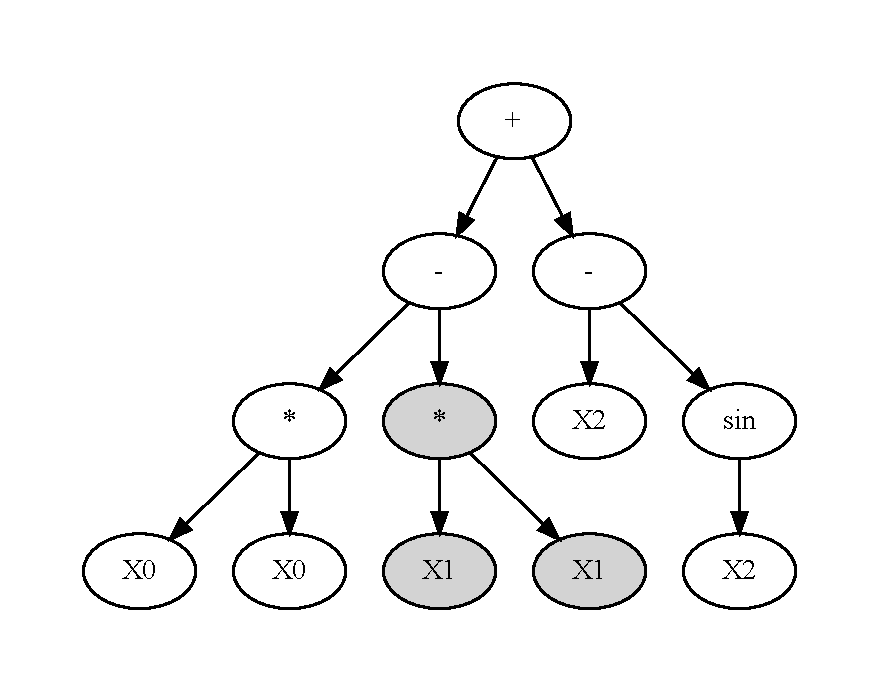
\includegraphics[scale=0.23]{images/graphviz/hoist_mut_before.dot.pdf}
          \caption{Original expression tree.}
          \label{fig:hoist_muta}
        \end{subfigure}%
        \\
        \begin{subfigure}{0.6\textwidth}
          \centering
          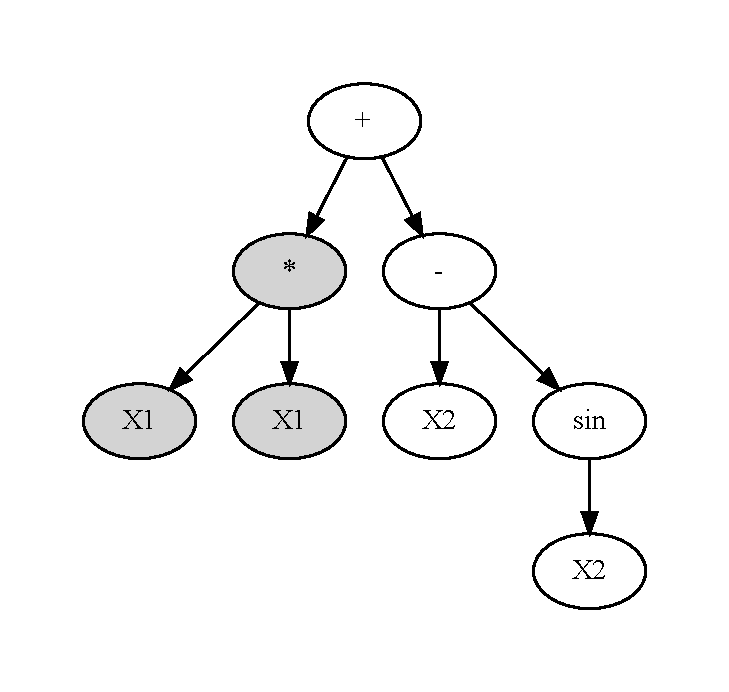
\includegraphics[scale=0.23]{images/graphviz/hoist_mut_after.dot.pdf}
          \caption{Tree after hoist mutation.}
          \label{fig:hoist_mutb}
        \end{subfigure}
        \caption{Visualizing hoist mutations.}
        \label{fig:hoist}
      \end{figure}
    \end{column}
  \end{columns}
\end{frame}

\begin{frame}
  \frametitle{Point Mutations}
  \begin{itemize}
    \item For every node: 
    \begin{itemize}
      \item With a given probability, replace node with another node of the same arity
    \end{itemize}
    \item Each node is considered independent of the other.
  \end{itemize}
  Point mutations reintroduce extinct functions and help maintain diversity.
\end{frame}

\subsection{Existing Work}
\begin{frame}
  \frametitle{Existing Work}
  \Cref{tab:otherlibs} lists some popular GP libraries. Our implementation follows the mutation definitions of \texttt{gplearn}. 
  \begin{table}
    \begin{center}
      \begin{tabular}[c]{ccc}
        \toprule
        \textbf{Framework} &   \textbf{Language} & \textbf{Compute Type} \\
        \midrule
        KarooGP & Python & CPU/GPU \\
        TensorGP & Python & CPU/GPU \\
        DEAP & Python & CPU \\
        gplearn  & Python & CPU \\
        ECJ & Java & CPU \\
        \bottomrule
      \end{tabular}
      \caption{Existing GP frameworks along with language and device support}
      \label{tab:otherlibs}
    \end{center}
  \end{table}
\end{frame}

%------------------------------------------------
\section{Our Contributions}
%------------------------------------------------

\subsection{Representation \& Memory Footprint}
\begin{frame}
  \frametitle{Representation \& Memory Footprint}
  \begin{itemize}
    \item Programs are represented in an Array of Structures (AoS) format.
    \item Evaluated in GPU using a thread local stack of maximum size $20$.
    \item History of programs for all generations is maintained on the CPU. 
    \item GPU stores only $2$ program populations, which is updated in a ping-pong fashion in every generation.
  \end{itemize}
\end{frame}

%------------------------------------------------

\subsection{Our Parallelization Strategy}
\begin{frame}
  \frametitle{The Parallel GP Algorithm}
  The Selection and Evaluation steps are parallelized using the GPU. The changes with respect to the classical algorithm are as follows:
  \begin{enumerate}
    \item Selection --- Parallelized tournament selection is used to determine next generation programs.
    \item Mutations --- The donor subtree in crossover is continuously hoisted until the child tree satisfies maximum depth requirements.
    \item Evaluation --- Split into an execution and a fitness computation phase. Both phases are completely vectorized using CUDA kernels.
  \end{enumerate}
\end{frame}

\begin{frame}
  \frametitle{Tournament Selection}
  \begin{itemize}
    \item For a given tournament thread:
      \begin{itemize}
        \item Select $k$ random programs from the population.
        \item Find the optimal program among selected programs based on fitness criterion.
        \item Mark optimal program as the current thread's winner.
      \end{itemize}
    \item We manually apply branch predication to avoid thread divergence when finding the optimal program in our implementation.
  \end{itemize}
\end{frame}

\begin{frame}
  \frametitle{Evaluation}
  \begin{itemize}
    \item Split into $2$ phases, execution and fitness computation. 
    \item Accounts for $71 \%$ of training time on average.
    \item Execution is parallelized across all dataset rows and program population - predicted values for every row and program are computed in this step.
    \item Fitness Computation sets program fitness values using the loss metric between the predicted and actual values. 
  \end{itemize}
\end{frame}

\begin{frame}
  \frametitle{Execution}
  \begin{itemize}
    \item For a given program:
      \begin{itemize}
        \item For a given dataset row:
          \begin{itemize}
            \item Execute program on row and produce predicted output.
            \item Record predicted output for given program.
          \end{itemize}
      \end{itemize}
    \item The above process is implemented using a CUDA kernel, where every thread corresponds to a unique thread and row. 
    \item Stack operations are carried out using unrolled loops to avoid possible indirect global memory access (using the current number of stack elements).
    \item Every thread in a  thread-block has to execute the same program in order to avoid warp divergence.
  \end{itemize}
\end{frame}

\begin{frame}
  \frametitle{Fitness Computation}
  \begin{itemize}
    \item Computed between predicted and actual values per program. 
    \item Actual values are broadcasted along across population dimension during loss computation.
    \item Weighted version of the following loss functions are supported (using \texttt{raft} linalg primitives)
      \begin{itemize}
        \item Mean Absolute Error (MAE) --- default
        \item Mean Square Error (MSE)
        \item Root Mean Square Error (RMSE)
        \item Logistic Loss (Only binary loss)
        \item Karl Pearson's Correlation Coefficient 
        \item Spearman's Rank Correlation Coefficient
      \end{itemize}
  \end{itemize}
    
\end{frame}

%------------------------------------------------

\subsection{Challenges}
\begin{frame}
  \frametitle{Avoiding Thread Divergence}
  \begin{itemize}
    \item Manual branch predication is used to unroll nested \lstinline!if! blocks in tournament selection kernel. This is necessary since each tournament thread in a warp can have different winners.
    \item We ensure that every thread-block of execution kernel executes the same program. This ensures same execution paths for all warp threads. 
  \end{itemize}
\end{frame}

\begin{frame}[fragile]
  \centering
  \frametitle{Memory Transfers}
  \begin{itemize}
    \item Nested copy problem due to the presence of the \lstinline!nodes! pointer inside every program. 
    \item Continuous allocation and deallocation of GPU memory for storing prefix list in every generation.
  \end{itemize}
\begin{minipage}{0.5\textwidth}
  \centering
  \begin{lstlisting}[caption={Simplified code for program struct},label={lst:programstruct}]
  struct program {
    node *nodes;
    int len;
    int depth;
    float raw_fitness_;
    metric_t metric;
    mutation_t mut_type;
  }; 
\end{lstlisting}
\end{minipage}
\begin{minipage}{0.4\textwidth}
  We need atleast $2$ \lstinline!cudaMemcpy! calls to copy the given program struct to the GPU.
\end{minipage}
\end{frame}
%------------------------------------------------
\section{Experimental Results}
%------------------------------------------------

\subsection{Setup}
\begin{frame}
  \frametitle{What do we benchmark?}
  Since GP still doesn't have standardized benchmarks, we use synthetic datasets for producing all results.
  \begin{itemize}
    \item We compare average execution time for $5$ GP libraries -- \texttt{cuML}, \texttt{gplearn}, \texttt{KarooGP(GPU)}, \texttt{TensorGP(CPU)}, \texttt{TensorGP(GPU)}
    \item We visualize the variation of training fitness across generations with increasing dataset size for \texttt{cuML}
    \item We compare the evolution of fitness values for \texttt{cuML} and \texttt{gplearn}. 
  \end{itemize}
\end{frame}

\begin{frame}
  \frametitle{The Regression Problem}
  In all the following benchmarks, the main goal is to generate a program which computes (or approximates) the Pagie Polynomial.
  \begin{block}{Pagie Polynomial}
    \begin{align*}
      f(x,y) = \frac{1}{1 + x^{-4}} + \frac{1}{1 + y^{-4}}
    \end{align*}  
  \end{block}
  Symbolic Regressors are trained on $7$ synthetic datasets ranging in size from $4096$ to $16$ million rows, where $(x,y) \in [-5,5]^2$ for all datasets.
\end{frame}

\begin{frame}
  \frametitle{Common Parameters}
  % Table
  \begin{table}
    \small
    \begin{tabular}[c]{cc}
      \toprule
      \textbf{Parameter} & \textbf{Value} \\
      \midrule
      Runs                      & 10      \\
      Number of Generations     & 50      \\
      Population size           & 50      \\
      Tournament size           & 4       \\ 
      Generation Method         & Ramped half-and-half \\
      Fitness Metric            & RMSE    \\
      Crossover probability     & 0.7     \\
      Mutation probability      & 0.25    \\
      Reproduction probability  & 0.05    \\
      Domain range              & [-5,5]  \\
      Function Set              & $\{+,-,*,\div,\sin ,\cos,\tan\}$ \\
      \bottomrule
    \end{tabular}
    \caption{Common parameters used for comparing execution time across libraries}
    \label{tab:params}
  \end{table}
\end{frame}
%------------------------------------------------

\subsection{Execution Time}
\begin{frame}
  \frametitle{Comparing Execution Time}
  % Graph
  \begin{figure}[ht]
    \centering
    \includegraphics[scale=0.329]{images/ExecutionTimesV100.pdf}
    \caption{Log-Log Plot of Execution Time for various libraries. The number of rows considered exponentially increases from $4096$ to $16$ million.}
    \label{fig:exectimes}
  \end{figure}
\end{frame}

\begin{frame}
  \frametitle{Comparing Execution Time($2$)}
  % Table
  \begin{table}
    \tiny
    \begin{tabular}{llrrrrrrr}
      \toprule
      \texttt{NumRows} & {} &  4096.00 &  16384.00 &  65536.00 & 262144.00 & 1048576.00 & 4194304.00 & 16777216.00 \\
      \midrule
      \texttt{cuml} & mean &   0.163 &    0.242 &    0.294 &    0.444 &    1.357 &    5.840 &    13.467 \\
                  & std &     5e-4 &      1.8e-3 &      4.9e-3 &      2.1e-3 &       7.2e-3 &       7.9e-3 &        5.9e-3 \\
      \texttt{gplearn} & mean &  1.79 &   2.27 &   4.69 &  19.04 &   97.18 &  522.97 &         NaN \\
                  & std &    4.46e-2 &      8.9e-3 &     2.12e-2 &     0.85 &     0.161 &    1.69 &         NaN \\
      \texttt{KarooGP} & mean & 75.58 & 111.94 & 114.57 & 184.012 &  474.93 &        NaN &         NaN \\
                  & std & 11.29 &  63.72 &  62.67 &  61.89 &  104.03 &        NaN &         NaN \\
      \texttt{TensorGP}\footnotemark & mean &  6.12 &   5.75 &   4.94 &   5.40 &    4.39 &    7.22 &    17.68 \\
                  & std &  1.09 &    0.23 &    0.185 &    0.40 &     0.29 &     0.21 &      0.37 \\
      \texttt{TensorGP}\footnotemark & mean &  2.53 &   6.94 &   7.47 &  16.78 &   46.14 &  125.70 &         NaN \\
                  & std &   0.25 &    0.10 &    0.12 &     5.7e-2 &     0.22 &     0.75 &         NaN \\
      \bottomrule
      \end{tabular}      
    \caption{Table containing mean and standard deviation of execution time across $10$ runs in seconds across different libraries. NaN denotes that the test timed out after $2$ hours.}
    \label{tab:execavgs}
  \end{table}
  \footnotetext[1]{GPU}
  \footnotetext[2]{CPU}
\end{frame}

%------------------------------------------------

\subsection{Fitness}
\begin{frame}
  \frametitle{Fitness with increasing dataset size.}
  % Graph
  \begin{figure}[htbp]
    \centering
    \includegraphics[scale=0.4]{images/RMSErrorV100.pdf}
    \caption{Plot showcasing the variation of Root Mean Square(RMS) error of with the number of generations. The error value corresponds to the fitness value of the optimal tree in every generation. }
    \label{fig:besttrainfit}
  \end{figure}
\end{frame}

% \begin{frame}
%   \frametitle{Comparing fitness evolution with \texttt{gplearn}}
%   % Graph
%   \begin{figure}[ht]
%     \centering
%     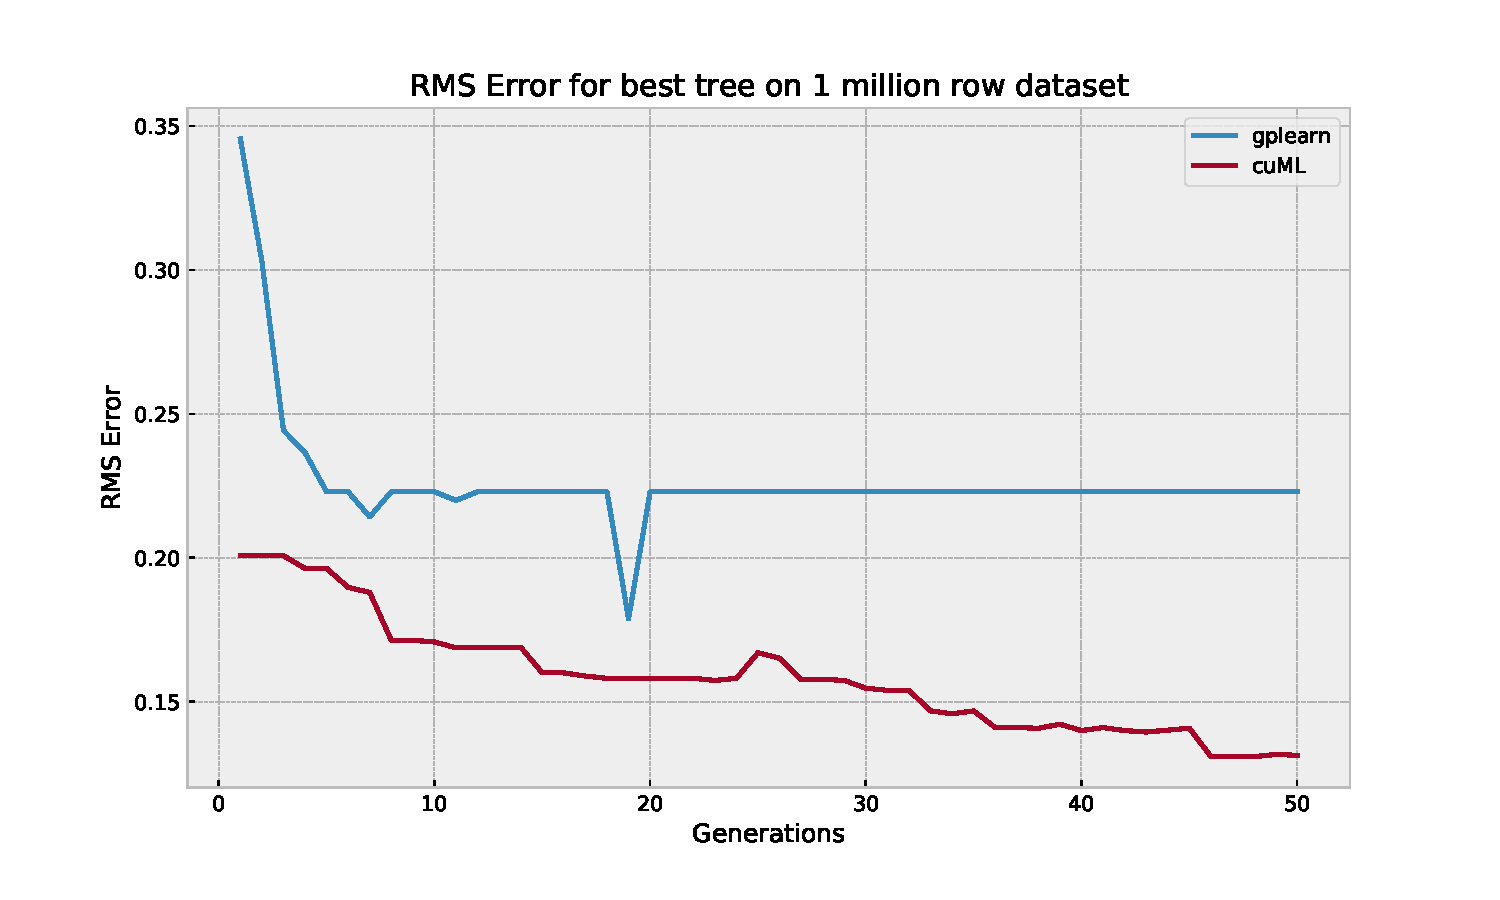
\includegraphics[scale=0.4]{images/RMSErrorGPLEARN.pdf}
%     \caption{Plot showcasing variation of the best tree fitness(during training) with number of generations for both \texttt{cuML} and \texttt{gplearn}. The fitness values correspond to the $1$ million row dataset for both libraries.}
%     \label{fig:gplearnvscuML1mil}
%   \end{figure}
% \end{frame}
%------------------------------------------------
\section{Conclusion}
\begin{frame}
  \frametitle{Concluding Remarks}
  \begin{itemize}
    \item \texttt{cuML} is faster compared to all other standard libraries for symbolic regression (and by extension, classification and transformation).
    \item We achieve an average speedup of $40\times$ w.r.t. \texttt{gplearn}, a CPU parallelized GP library which serves as a base for our code.
    \item There is still scope for further optimization and improvement.
  \end{itemize}
\end{frame}

\begin{frame}
  \frametitle{Further Optimizations}
  \begin{itemize}
    \item Balancing the program trees stored in the GPU
    \item Converting the program list into a DAG to cache repeated computations --- will need a new representation and evaluation scheme.
  \end{itemize}
  \begin{figure}
    \centering
    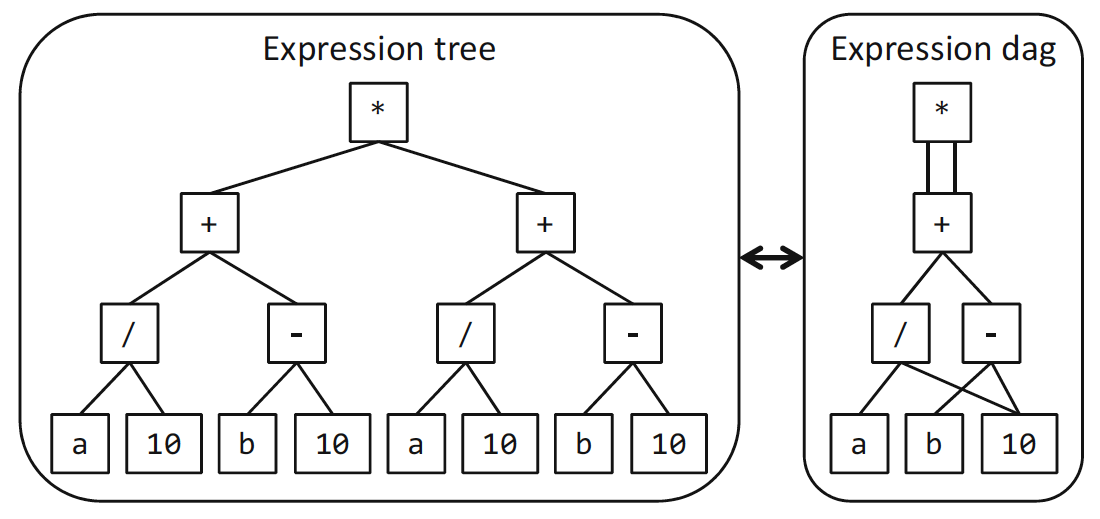
\includegraphics[scale=0.22]{images/dag.png}
    \caption{Example for tree to DAG conversion\footnotemark.}
  \end{figure}
  \footnotetext[1]{Figure taken from Westfechtel, Bernhard. ``Case-based exploration of bidirectional transformations in QVT Relations.'' Software \& Systems Modeling (2016): 1-41}
\end{frame}

\begin{frame}
  \frametitle{New Features}
  \begin{itemize}
    \item Support for custom function sets --- function pointers/lambdas
    \item Supporting custom loss functions --- \lstinline!__device__! lambda functions for pre-processing, reduction and post-processing operations.
  \end{itemize}
\end{frame}

\begin{frame}
\Huge{\centerline{Fin}}
% \Huge{Fin}
% \begin{center}
%   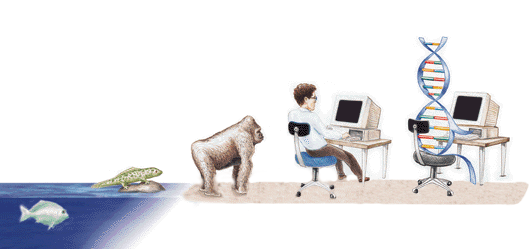
\includegraphics[scale=0.5]{images/evolution.png}
% \end{center}
\end{frame}

% %----------------------------------------------------------------------------------------

\end{document} 